%!TEX encoding = UTF-8 Unicode
\documentclass[onecolumn,12pt]{book}
\usepackage[english,italian]{babel}
\usepackage{inconsolata}
%\renewcommand*\familydefault{\ttdefault} %% Only if the base font of the document is to be typewriter style
\usepackage[T1]{fontenc}

\usepackage{a4wide,Sweave,url}
\usepackage{verbatim}
\usepackage{makeidx}
\usepackage{babelbib}
\usepackage{float}
\usepackage{fancyhdr}
\usepackage[T1]{fontenc}
\usepackage[utf8]{inputenc}
\usepackage{framed}
\usepackage{lipsum}
\usepackage[dvipsnames]{color}
\definecolor{shadecolor}{rgb}{0.9,0.9,0.9}
\usepackage{graphicx}
\usepackage{fancyvrb}
\usepackage{amsmath}
\usepackage{Sweave}
\usepackage{hyperref}
\newenvironment{question}{\item \textbf{Esercizio}\newline}{}
\newenvironment{solution}{\textbf{Soluzione}\newline}{}
\newenvironment{answerlist}{\renewcommand{\labelenumi}{(\alph{enumi})}\begin{enumerate}}{\end{enumerate}}
\definecolor{grigetto}{rgb}{0.9,0.9,0.9}
 
\DefineVerbatimEnvironment{Sinput}{Verbatim} {xleftmargin=2em} \DefineVerbatimEnvironment{Soutput}{Verbatim}{xleftmargin=2em} \DefineVerbatimEnvironment{Scode}{Verbatim}{xleftmargin=2em} \fvset{listparameters={\setlength{\topsep}{0pt}}} \renewenvironment{Schunk}{\small\vspace{\topsep}}{\vspace{\topsep}\normalsize}
\lhead[\thepage]{\today}
%\usepackage{draftwatermark}
\usepackage{wrapfig}
\usepackage{listings}
\pagestyle{fancy}
\newcounter{fnotes}\setcounter{fnotes}{1}
\newcounter{Raction}\setcounter{Raction}{1}
\newcommand{\varia}[1]{\textsl{\textsf{#1}}}
\newcommand{\mytilde}{$\sim$}
\newcommand{\maurizio}[1]{\color{red}#1 \color{black}}
\newcommand{\federico}[1]{\color{green}#1 \color{black}}
 %\newenvironment{question}{\item \textbf{Problema}\newline}{}
%\newenvironment{solution}{\textbf{Soluzione}\newline}{}
%\DefineVerbatimEnvironment{Sinput}{Verbatim} {xleftmargin=2em,
                                            %  frame=single}
\DefineVerbatimEnvironment{Soutput}{Verbatim}{xleftmargin=2em,   frame=single}
 \newenvironment{ese} [1]{\vskip10pt
%\begin{center}
%\begin{minipage}{12cm}
 \markright{\today}
\definecolor{grigetto}{rgb}{0.9,0.9,0.9}
\colorbox{grigetto}{\parbox{\linewidth}{#1}}}
                          {
                         % \end{minipage}
                          %\end{center}
                          \medskip}
 \newcommand{\virgolette}{\selectlanguage{english}\texttt{"}\selectlanguage{italian}}
 \frontmatter\title{Matematica e Statistica con \textsf{R}}
\author{Federico Comoglio e  Maurizio Rinaldi}
\markright{\today}
\lhead{\today}
\renewcommand{\chaptermark}[1]{%
 \markboth{\chaptername
 \ \thechapter.\ #1}{}}
%\renewcommand{\sectionmark}[1]{%
% \markboth{\sectionname
% \ \thesection.\ #1}{}}
\newcommand{\rst}{\textsf{RStudio}~}
\newcommand{\rpr}{\textsf{R}~}
\makeindex
\begin{document}
\setkeys{Gin}{width=0.7\textwidth}
\SweaveOpts{concordance=TRUE}
\markright{\today}
\thispagestyle{empty}
\maketitle
\newpage
\thispagestyle{empty}
\tableofcontents
\newpage
\thispagestyle{empty}
 \mainmatter

\chapter{Introduzione}
Per accedere ai dati richiesti in questa parte occorre caricare il pacchetto allegato \texttt{libroR}. Per farlo conviene scaricare il file \texttt{libroR$\_0$.0.tgz}  sul proprio computer e  selezionare il menu \texttt{Install}
\begin{center}\begin{figure}[H]
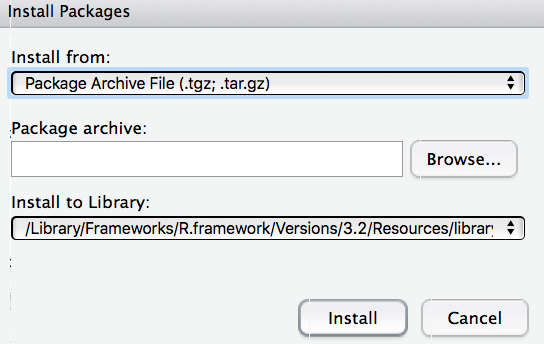
\includegraphics[width=0.4\textwidth]{../grafici/installlibro.png}
\caption{Procedura di installazione del pacchetto}
\label{fig::rlibroinstall} \end{figure}
\end{center}
Il file viene poi localizzato usando \texttt{Browse..}. \\
Alternativamente si pu\`o utilizzare direttamente il comando

\begin{knitrout}
\definecolor{shadecolor}{rgb}{0.969, 0.969, 0.969}\color{fgcolor}\begin{kframe}
\begin{alltt}
\hlkwd{install.packages}\hlstd{(}\hlstr{"libroR_0.0.tgz"}\hlstd{,} \hlkwc{repos} \hlstd{=} \hlkwa{NULL}\hlstd{,} \hlkwc{type} \hlstd{= .Platform}\hlopt{$}\hlstd{pkgType)}
\end{alltt}
\end{kframe}
\end{knitrout}
a patto di impostare la \emph{working directory} precisamente dove si trova il file.
Il pacchetto va poi successivamente caricato con il comando
\begin{knitrout}
\definecolor{shadecolor}{rgb}{0.969, 0.969, 0.969}\color{fgcolor}\begin{kframe}
\begin{alltt}
\hlkwd{library}\hlstd{(}\hlstr{"libroR"}\hlstd{)}
\end{alltt}


{\ttfamily\noindent\itshape\color{messagecolor}{\#\# \\\#\# Attaching package: 'libroR'}}

{\ttfamily\noindent\itshape\color{messagecolor}{\#\# The following objects are masked from 'package:EsamiR':\\\#\# \\\#\#\ \ \ \  meteo, studenti}}\end{kframe}
\end{knitrout}

Precisiamo inoltre che questa \`e una versione assolutamente preliminare.
\chapter{Strutture di dati}

 
Per visualizzare un oggetto di \textsf{R} si pu\`o usare il comando \texttt{print} o il comando \texttt{cat} che fornisce spesso un risultato migliore. \texttt{str} visualizza la struttura di un oggetto mentre \texttt{head} o \texttt{tail} ne visualizzano l'inizio o la fine.


\section{I diversi  tipi di vettori}
\subsection{Vettori di caratteri/stringhe}
Una stringa\index{stringa} di testo \`e una collezione di caratteri; in genere, una stringa \`e resa riconoscibile dall'essere racchiusa tra virgolette.
\subsubsection{Operare con le stringhe}
Oltre alle virgolette, vi sono numerosi altri caratteri speciali che possono apparire in una stringa.
I pi\`u comuni sono ``\texttt{\textbackslash t}'' per \texttt{TAB}, `` \texttt{\textbackslash n}'' per una nuova linea e ``\texttt{\textbackslash }'' per un singolo {\it backslash}.
Quest'ultimo carattere \`e un carattere di \emph{escape} e consente una lettura diversa di quanto lo segue.  Per esempio
\begin{knitrout}
\definecolor{shadecolor}{rgb}{0.969, 0.969, 0.969}\color{fgcolor}\begin{kframe}
\begin{alltt}
\hlkwd{cat}\hlstd{(}\hlstr{"\textbackslash{}"sin\textbackslash{}""}\hlstd{)}
\end{alltt}
\begin{verbatim}
## "sin"
\end{verbatim}
\begin{alltt}
\hlkwd{nchar}\hlstd{(}\hlstr{"\textbackslash{}"sin\textbackslash{}""}\hlstd{)}
\end{alltt}
\begin{verbatim}
## [1] 5
\end{verbatim}
\begin{alltt}
\hlkwd{cat}\hlstd{(}\hlstr{"\textbackslash{}\textbackslash{}"}\hlstd{)}
\end{alltt}
\begin{verbatim}
## \
\end{verbatim}
\begin{alltt}
\hlkwd{cat}\hlstd{(}\hlstr{"ora a capo\textbackslash{}nsono a capo?"}\hlstd{)}
\end{alltt}
\begin{verbatim}
## ora a capo
## sono a capo?
\end{verbatim}
\begin{alltt}
\hlkwd{cat}\hlstd{(}\hlstr{"ora spazio\textbackslash{}triprendo"}\hlstd{)}
\end{alltt}
\begin{verbatim}
## ora spazio	riprendo
\end{verbatim}
\end{kframe}
\end{knitrout}
La funzione \texttt{nchar}, \index{\texttt{nchar}} che conta il numero di caratteri di una stringa, non includer\`a quindi il carattere di \emph{escape}\index{\emph{escape}} nel totale dei caratteri. Ad esempio:
\begin{knitrout}
\definecolor{shadecolor}{rgb}{0.969, 0.969, 0.969}\color{fgcolor}\begin{kframe}
\begin{alltt}
\hlstr{"Tab\textbackslash{}t"}
\end{alltt}
\begin{verbatim}
## [1] "Tab\t"
\end{verbatim}
\begin{alltt}
\hlkwd{cat}\hlstd{(}\hlstr{"Tab\textbackslash{}t"}\hlstd{)}
\end{alltt}
\begin{verbatim}
## Tab	
\end{verbatim}
\begin{alltt}
\hlkwd{nchar}\hlstd{(}\hlstr{"Tab\textbackslash{}t"}\hlstd{)}
\end{alltt}
\begin{verbatim}
## [1] 4
\end{verbatim}
\end{kframe}
\end{knitrout}



Succede spesso di dover lavorare in modo automatico con stringhe di testo, anche nello scrivere indirizzi di rete o cartelle di lavoro. In  \textsf{R} diversi comandi consentono la  generazione, manipolazione e stampa di una o pi\`u stringhe di testo\footnote{Per un  uso pi\`u specifico si pu\`o consultare il pacchetto \texttt{biostrings}.}. Consideriamo inizialmente una singola frase.
%codechunk
\begin{knitrout}
\definecolor{shadecolor}{rgb}{0.969, 0.969, 0.969}\color{fgcolor}\begin{kframe}
\begin{alltt}
\hlstd{x}\hlkwb{=}\hlstr{"lavorare con le stringhe"}
\end{alltt}
\end{kframe}
\end{knitrout}
Possiamo verificarne la classe e determinare il numero di caratteri di \texttt{x}
%codechunk
\begin{knitrout}
\definecolor{shadecolor}{rgb}{0.969, 0.969, 0.969}\color{fgcolor}\begin{kframe}
\begin{alltt}
\hlkwd{class}\hlstd{(x)}
\end{alltt}
\begin{verbatim}
## [1] "character"
\end{verbatim}
\begin{alltt}
\hlkwd{nchar}\hlstd{(x)}
\end{alltt}
\begin{verbatim}
## [1] 24
\end{verbatim}
\end{kframe}
\end{knitrout}
e anche considerare sottostringhe
%codechunk
\begin{knitrout}
\definecolor{shadecolor}{rgb}{0.969, 0.969, 0.969}\color{fgcolor}\begin{kframe}
\begin{alltt}
\hlkwd{substr}\hlstd{(x,}\hlnum{3}\hlstd{,}\hlnum{8}\hlstd{)}
\end{alltt}
\begin{verbatim}
## [1] "vorare"
\end{verbatim}
\end{kframe}
\end{knitrout}
o  abbreviazioni ottenibili con il comando \texttt{abbreviate} \index{\texttt{abbreviate}}
%codechunk
\begin{knitrout}
\definecolor{shadecolor}{rgb}{0.969, 0.969, 0.969}\color{fgcolor}\begin{kframe}
\begin{alltt}
\hlkwd{abbreviate}\hlstd{(}\hlstr{"Mario Rossi"}\hlstd{,}\hlnum{4}\hlstd{)}
\end{alltt}
\begin{verbatim}
## Mario Rossi 
##      "MrRs"
\end{verbatim}
\end{kframe}
\end{knitrout}

Certi oggetti possono essere convertiti a stringhe: per esempio il numero 2 pu\`o essere visto come una stringa e riconvertito a numero.
%codechunk
\begin{knitrout}
\definecolor{shadecolor}{rgb}{0.969, 0.969, 0.969}\color{fgcolor}\begin{kframe}
\begin{alltt}
\hlstd{i}\hlkwb{=}\hlnum{2}\hlstd{;}\hlkwd{toString}\hlstd{(i)}
\end{alltt}
\begin{verbatim}
## [1] "2"
\end{verbatim}
\begin{alltt}
\hlkwd{as.numeric}\hlstd{(}\hlkwd{toString}\hlstd{(i))}
\end{alltt}
\begin{verbatim}
## [1] 2
\end{verbatim}
\end{kframe}
\end{knitrout}
Alcune stringhe molto frequenti sono le lettere \index{\texttt{letters}}\index{\texttt{LETTERS}} dell'alfabeto, maiuscole o minuscole
%codechunk
\begin{knitrout}
\definecolor{shadecolor}{rgb}{0.969, 0.969, 0.969}\color{fgcolor}\begin{kframe}
\begin{alltt}
\hlstd{letters[}\hlnum{1}\hlopt{:}\hlnum{10}\hlstd{]}
\end{alltt}
\begin{verbatim}
##  [1] "a" "b" "c" "d" "e" "f" "g" "h" "i" "j"
\end{verbatim}
\begin{alltt}
\hlstd{LETTERS[}\hlnum{1}\hlopt{:}\hlnum{10}\hlstd{]}
\end{alltt}
\begin{verbatim}
##  [1] "A" "B" "C" "D" "E" "F" "G" "H" "I" "J"
\end{verbatim}
\end{kframe}
\end{knitrout}
o i mesi dell'anno (per esempio abbreviati in inglese)\index{\texttt{month.abb}}
%codechunk

\begin{knitrout}
\definecolor{shadecolor}{rgb}{0.969, 0.969, 0.969}\color{fgcolor}\begin{kframe}
\begin{alltt}
\hlstd{month.abb}
\end{alltt}
\begin{verbatim}
##  [1] "Jan" "Feb" "Mar" "Apr" "May" "Jun" "Jul" "Aug" "Sep"
## [10] "Oct" "Nov" "Dec"
\end{verbatim}
\end{kframe}
\end{knitrout}
Le stringhe possono poi essere ``incollate'' con il comando\index{\texttt{paste}}
%codechunk
\begin{knitrout}
\definecolor{shadecolor}{rgb}{0.969, 0.969, 0.969}\color{fgcolor}\begin{kframe}
\begin{alltt}
\hlkwd{paste}\hlstd{(}\hlstr{"a"}\hlstd{,}\hlstr{"b"}\hlstd{,}\hlkwc{sep}\hlstd{=}\hlstr{""}\hlstd{)}
\end{alltt}
\end{kframe}
\end{knitrout}
dove \texttt{sep}  indica il separatore usato.
E tutto insieme
%codechunk


\begin{knitrout}
\definecolor{shadecolor}{rgb}{0.969, 0.969, 0.969}\color{fgcolor}\begin{kframe}
\begin{alltt}
\hlkwa{for} \hlstd{(i} \hlkwa{in} \hlnum{1}\hlopt{:}\hlnum{5}\hlstd{)} \hlkwd{cat}\hlstd{(}\hlkwd{paste}\hlstd{(}\hlstr{"a"}\hlstd{,}\hlkwd{toString}\hlstd{(i),}\hlstr{"\textbackslash{}t"}\hlstd{,}\hlkwc{sep}\hlstd{=}\hlstr{""}\hlstd{))}
\end{alltt}
\begin{verbatim}
## a1	a2	a3	a4	a5	
\end{verbatim}
\end{kframe}
\end{knitrout}
Il comando pu\`o anche essere utilizzato su vettori.
Per esempio
%codechunk
\begin{knitrout}
\definecolor{shadecolor}{rgb}{0.969, 0.969, 0.969}\color{fgcolor}\begin{kframe}
\begin{alltt}
\hlkwd{paste}\hlstd{(letters[}\hlnum{1}\hlopt{:}\hlnum{10}\hlstd{],}\hlnum{1}\hlopt{:}\hlnum{10}\hlstd{,}\hlkwc{sep}\hlstd{=}\hlstr{""}\hlstd{)}
\end{alltt}
\begin{verbatim}
##  [1] "a1"  "b2"  "c3"  "d4"  "e5"  "f6"  "g7"  "h8"  "i9" 
## [10] "j10"
\end{verbatim}
\end{kframe}
\end{knitrout}
La \textit{recycling rule} continua a valere
%codechunk

\begin{knitrout}
\definecolor{shadecolor}{rgb}{0.969, 0.969, 0.969}\color{fgcolor}\begin{kframe}
\begin{alltt}
\hlkwd{paste}\hlstd{(letters[}\hlnum{1}\hlopt{:}\hlnum{3}\hlstd{],}\hlnum{1}\hlopt{:}\hlnum{10}\hlstd{,}\hlkwc{sep}\hlstd{=}\hlstr{""}\hlstd{)}
\end{alltt}
\begin{verbatim}
##  [1] "a1"  "b2"  "c3"  "a4"  "b5"  "c6"  "a7"  "b8"  "c9" 
## [10] "a10"
\end{verbatim}
\begin{alltt}
\hlkwd{paste}\hlstd{(letters[}\hlnum{1}\hlopt{:}\hlnum{3}\hlstd{],}\hlnum{1}\hlopt{:}\hlnum{12}\hlstd{,}\hlkwc{sep}\hlstd{=}\hlstr{""}\hlstd{)}
\end{alltt}
\begin{verbatim}
##  [1] "a1"  "b2"  "c3"  "a4"  "b5"  "c6"  "a7"  "b8"  "c9" 
## [10] "a10" "b11" "c12"
\end{verbatim}
\end{kframe}
\end{knitrout}
e giocando con \texttt{rep} si possono ottenere diverse combinazioni.
\begin{knitrout}
\definecolor{shadecolor}{rgb}{0.969, 0.969, 0.969}\color{fgcolor}\begin{kframe}
\begin{alltt}
\hlkwd{paste}\hlstd{(}\hlkwd{rep}\hlstd{(letters[}\hlnum{1}\hlopt{:}\hlnum{3}\hlstd{],}\hlkwc{each}\hlstd{=}\hlnum{5}\hlstd{),}\hlnum{1}\hlopt{:}\hlnum{15}\hlstd{,}\hlkwc{sep}\hlstd{=}\hlstr{""}\hlstd{)}
\end{alltt}
\begin{verbatim}
##  [1] "a1"  "a2"  "a3"  "a4"  "a5"  "b6"  "b7"  "b8"  "b9" 
## [10] "b10" "c11" "c12" "c13" "c14" "c15"
\end{verbatim}
\begin{alltt}
\hlkwd{paste}\hlstd{(}\hlkwd{rep}\hlstd{(letters[}\hlnum{1}\hlopt{:}\hlnum{3}\hlstd{],}\hlkwc{ntimes}\hlstd{=}\hlnum{5}\hlstd{),}\hlnum{1}\hlopt{:}\hlnum{15}\hlstd{,}\hlkwc{sep}\hlstd{=}\hlstr{""}\hlstd{)}
\end{alltt}
\begin{verbatim}
##  [1] "a1"  "b2"  "c3"  "a4"  "b5"  "c6"  "a7"  "b8"  "c9" 
## [10] "a10" "b11" "c12" "a13" "b14" "c15"
\end{verbatim}
\end{kframe}
\end{knitrout}
Con l'opzione \texttt{collapse="x"} le stringhe vengono unite con separatore la stringa "x".
%codechunk
\begin{knitrout}
\definecolor{shadecolor}{rgb}{0.969, 0.969, 0.969}\color{fgcolor}\begin{kframe}
\begin{alltt}
\hlkwd{paste}\hlstd{(}\hlkwd{c}\hlstd{(}\hlstr{"X"}\hlstd{,} \hlstr{"Y"}\hlstd{),} \hlnum{1}\hlopt{:}\hlnum{4}\hlstd{,} \hlkwc{sep} \hlstd{=} \hlstr{"-"}\hlstd{,} \hlkwc{collapse} \hlstd{=} \hlstr{"--"}\hlstd{)}
\end{alltt}
\begin{verbatim}
## [1] "X-1--Y-2--X-3--Y-4"
\end{verbatim}
\end{kframe}
\end{knitrout}
Si noti il separatore - dell'operazione \texttt{paste} e  - - dell'operazione \texttt{collapse}.

 \begin{shaded}
 \begin{enumerate}
 \item{} Inserisci il tuo cognome in una variabile `cognome' ed il tuo nome in una variabile 'nome'. Crea una terza variabile 'nomecognome' che contenga entrambi separati da un TAB. Stampa a console la scritta "Good job" seguita dal valore di nomecognome.
  \item{} Creare un elenco che contenga mesi e anno dal 2001 al 2010 nel seguente formato "tre lettere iniziali del mese-anno".
 \item{} Costruire una tabella che contenga tutte le parole di 2 lettere.
\item{}
Si consideri























































































